\documentclass{standalone}
\usepackage{pgfplots}
\pgfplotsset{compat=1.18}

\pgfplotsset{
    width=8.0cm,
    height=6.0cm,
    ticklabel style = {font=\small},
    grid=both, % major, minor, both
    major grid style={dashed, gray!30},
    minor grid style={dashed, gray!30},
    xlabel style={yshift=2mm, font=\small},
    ylabel style={yshift=-2mm, font=\small},
    legend style={font=\small, at={(0.50, 0.95)}, anchor=west, draw=none, fill=none},
    scale only axis=true,
}

\begin{document}

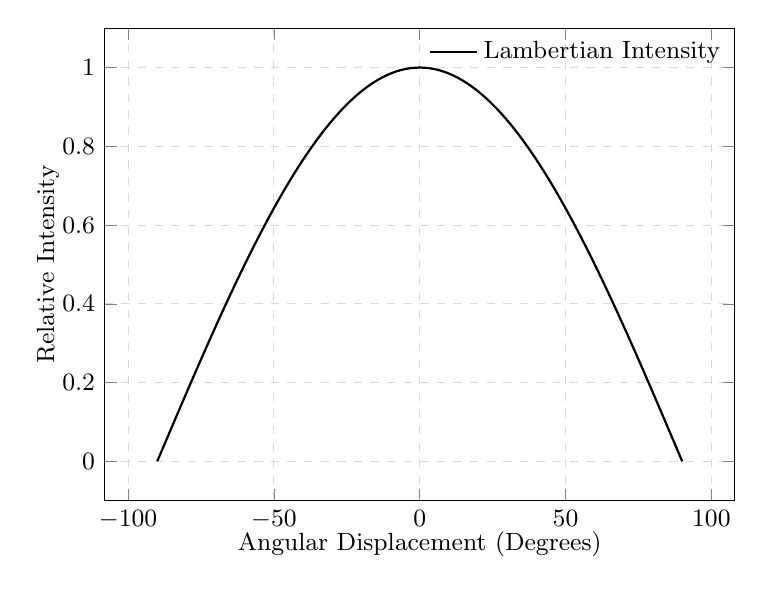
\begin{tikzpicture}
    \begin{axis}[
        xlabel={Angular Displacement (Degrees)},
        ylabel={Relative Intensity},
        domain=-90:90,
        samples=200,
    ]
        % Lambertian distribution
        \addplot[smooth, thick, black] {cos(x)}; 
        \legend{Lambertian Intensity}
    \end{axis}
\end{tikzpicture}

\end{document}
